\documentclass{article}
\usepackage{tikz}
\usetikzlibrary{arrows,shapes,positioning,shadows,trees}

\tikzset{
  basic/.style  = {draw, text width=2cm, drop shadow, font=\sffamily, rectangle},
  root/.style   = {basic, rounded corners=2pt, thin, align=center,
                   fill=orange!70},
  level 2/.style = {basic, rounded corners=6pt, thin,align=center, fill=orange!40,
                   text width=8em},
  level 3/.style = {basic, thin, align=left, fill=orange!20, text width=6.5em}
}

\begin{document}
  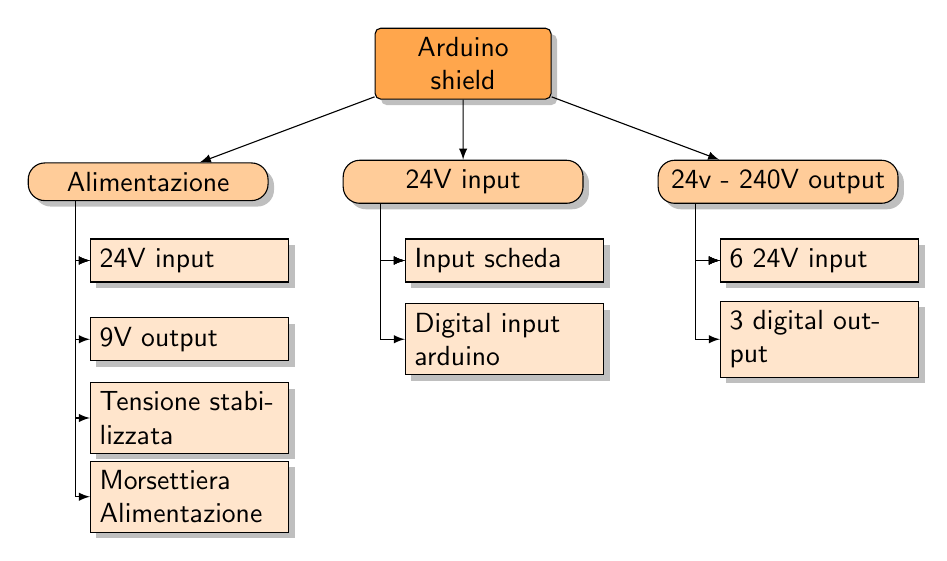
\begin{tikzpicture}[
            level 1/.style={sibling distance=40mm},
            edge from parent/.style={->,draw},
            >=latex]
          
          % root of the the initial tree, level 1
          \node[root] {Arduino shield}
          % The first level, as children of the initial tree
            child {node[level 2] (c1) {Alimentazione}}
            child {node[level 2] (c2) {24V input}}
            child {node[level 2] (c3) {24v - 240V output}};
          
          % The second level, relatively positioned nodes
          \begin{scope}[every node/.style={level 3}]
          \node [below of = c1, xshift=15pt] (c11) {24V input};
          \node [below of = c11] (c12) {9V output};
          \node [below of = c12] (c13) {Tensione stabilizzata};
          \node [below of = c13] (c14) {Morsettiera Alimentazione};
          
          \node [below of = c2, xshift=15pt] (c21) {Input scheda};
          \node [below of = c21] (c22) {Digital input arduino};
          
          
          \node [below of = c3, xshift=15pt] (c31) {6 24V input};
          \node [below of = c31] (c32) {3 digital output};
          \end{scope}
          
          % lines from each level 1 node to every one of its "children"
          \foreach \value in {1,2,3}
            \draw[->] (c1.195) |- (c11);
            \draw[->] (c1.195) |- (c12);
            \draw[->] (c1.195) |- (c13);
            \draw[->] (c1.195) |- (c14);
          
          \foreach \value in {1,...,4}
            \draw[->] (c2.195) |- (c21);
            \draw[->] (c2.195) |- (c22);
          
          \foreach \value in {1,...,5}
            \draw[->] (c3.195) |- (c31);
            \draw[->] (c3.195) |- (c32);

          \end{tikzpicture}
\end{document}
